\documentclass[11pt]{beamer}
\usetheme{Pittsburgh}
\usepackage[utf8]{inputenc}
\usepackage{amsmath}
\usepackage{amsfonts}
\usepackage{amssymb}
\usepackage{graphicx}
\author{Dom Owens}
\title{Nowcasting Under Structural Breaks}
%\setbeamercovered{transparent} 
%\setbeamertemplate{navigation symbols}{} 
%\logo{} 
%\institute{} 
%\date{} 
%\subject{} 
\begin{document}

\begin{frame}
\titlepage
\end{frame}

\begin{frame}
\tableofcontents
\end{frame}

\section{Overview}
\begin{frame}{Overview}
 
\begin{itemize}
	\item Fore/Now-casting GDP is useful
	\item GDP is observed at a low frequency
	\item We can use a factor model for x-casting
	\item Observed macro, survey, etc. data are often non-stationary
	\item Rolling windows are a naive way of dealing with this 
\end{itemize}

We will
\begin{itemize}
	\item Use a piecewise-stationary model
	\item Identify structural breaks with a new algorithm
	\item Use estimated break points intelligently for prediction
\end{itemize}
 
\end{frame}

\section{Model}
\begin{frame}{Model: Factors}
 For observations $\boldsymbol{X}_t \in \mathbb{R}^d$ we consider the factor model

\begin{equation} \label{factor model}
	\boldsymbol{X}_t = \boldsymbol{\chi}_t + \boldsymbol{\varepsilon}_t :=
	\boldsymbol{\Lambda} \boldsymbol{F}_t + \boldsymbol{\varepsilon}_t, \quad t = 1, \dots, n
\end{equation}
where $\boldsymbol{\chi}_t$ and $\boldsymbol{\varepsilon}_t$ are common and idiosyncratic components respectively.
 $\boldsymbol{F}_t \in \mathbb{R}^{r}$ is an unobservable vector of $r$ factors, $\boldsymbol{\Lambda} \in \mathbb{R}^{d \times r}$ is a fixed matrix of loadings, and $\boldsymbol{\varepsilon}_t$ are white noise.
${y}_{i,t} = \lambda^y_{i}{F}_{t} + {\varepsilon}^y_{i,t}$ is nowcasted series, observed at e.g. $t=1,4,7, \dots,$
\end{frame} 
 
\begin{frame}{Model: Piecewise-VAR} 

 Factors follow $VAR(p)$ with structural changes  
    $$
     {F}_{t}=\left\{\begin{array}{ll}
    {\boldsymbol{\Phi}_{1}\mathbb{F}_{t-1} + \boldsymbol{\eta}_{t},} & {k_0 = 1 \leq t \leq {k}_1} \\
    {\boldsymbol{\Phi}_{2}\mathbb{F}_{t-1} + \boldsymbol{\eta}_{t},} & {{k}_1 <t \leq {k}_2}  \\
    {\dots}                                                                                             \\ 
    {\boldsymbol{\Phi}_{q+1}\mathbb{F}_{t-1} + \boldsymbol{\eta}_{t},} & {{k}_{q} <t \leq {k}_{q+1}=n } 
    \end{array}\right. 
    $$
     $$  \boldsymbol{\Phi}_j = \left( \begin{array}{ll}  \boldsymbol{\Phi}_j^T(1)\\
        \dots \\
        \boldsymbol{\Phi}_j^T(r)
        \end{array}\right) \in \mathbb{R}^{r \times rp} 
        \quad \quad \mathbb{F}_{t-1} =\left[  \begin{array}{ll}
        \mathbb{F}_{t-1}(1) \\ 
        \ldots \\
        \mathbb{F}_{t-1}(r) \\
        \end{array}\right] \in \mathbb{R}^{ rp} % \nonumber 
    $$
where $\mathbb{F}_{t-1}(i) =\left[ F_{t-1}(i), \ldots, F_{t-p}(i)\right]^{T}$, and $\boldsymbol{\eta}_t$ are also white noise.
Change points are ${k}_j, j = 0, 1, \dots, q, q+1$ are unknown, to be estimated.
 
\end{frame}

\section{Change Point Analysis} 
\begin{frame}{Change Point Analysis} 
\begin{itemize}
	\item (1) identify the factor series using Principal Components Analysis (PCA) on $\boldsymbol{X}_t$
	\item (2) select first $\hat{r}$ components; $\hat{r}$ may be determined through some Information Criterion
	\item (3) run the $\texttt{mosumvar}$ algorithm on the resulting series
\end{itemize}
\end{frame}

\begin{frame}{Change Point Analysis: mosumvar} 
 Input: series $\{\boldsymbol{F}_t, t = 1, \dots, n \}$, bandwidth $G$
 
 At each $k= G,\dots, n-G$ calculate a test statistic $T_k$, comparing parameter estimates over window $k-G+1, \dots, k$ to window $k+1, \dots, k+G$. These will be large at change points, and small elsewhere. Use local maxima of series $\{T_k\}$ as location estimates.
 
 Output: Test outcome, Change point estimates
 
 
 \begin{figure}[h!]
	\centering
	%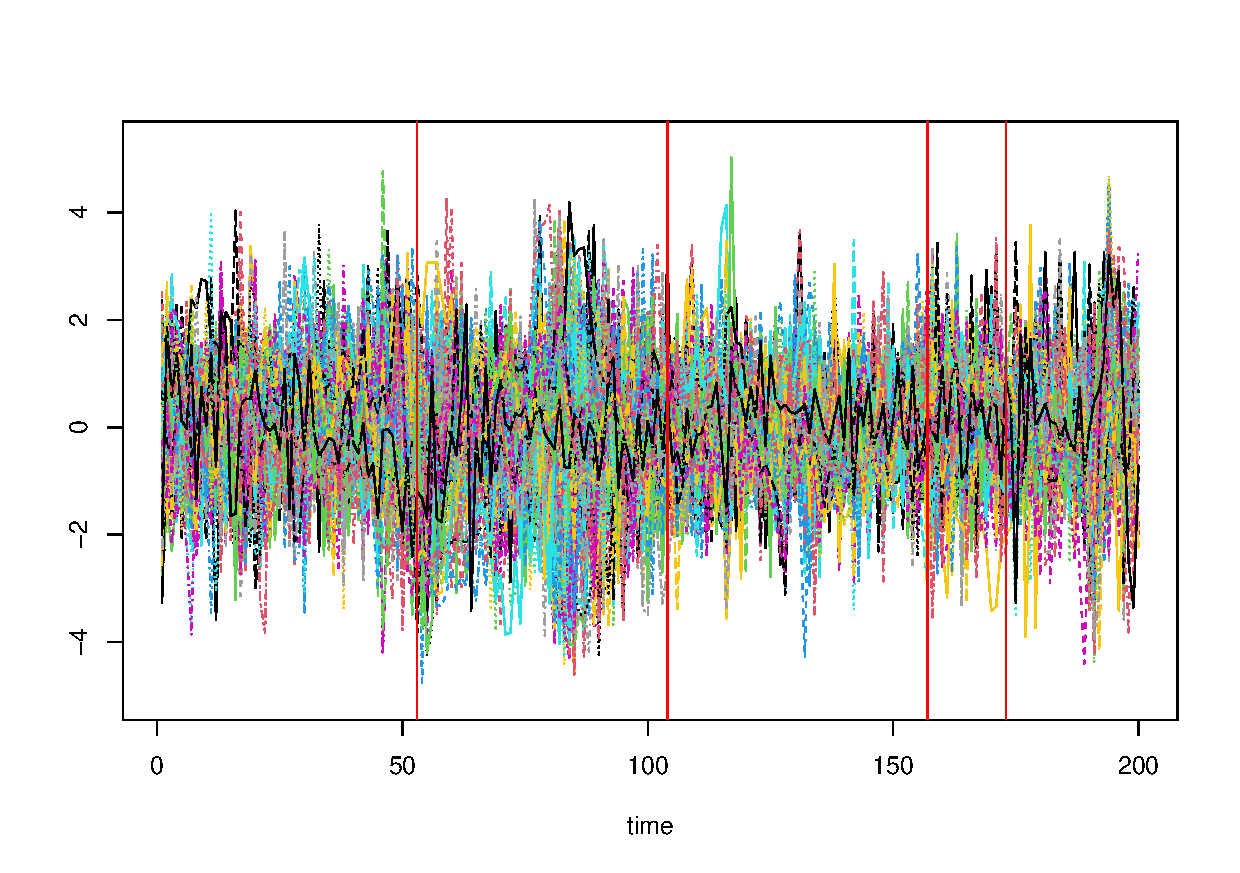
\includegraphics[scale=0.5]{datatscps.pdf}
	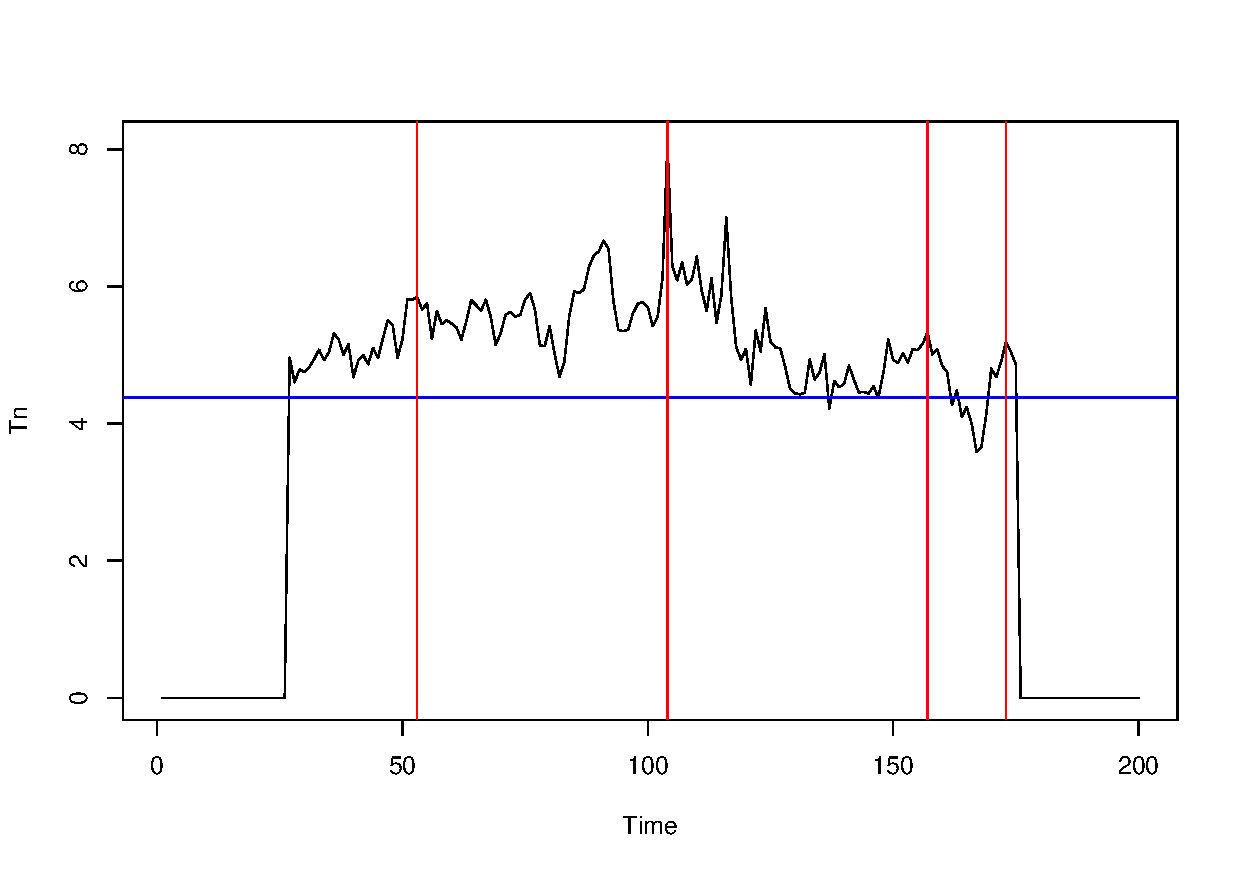
\includegraphics[scale=0.25]{app/datachangepoints.pdf}
 
\end{figure} 
\end{frame}


\begin{frame}{Change Point Analysis: Forecasting}
Having identified change points, how should we make predictions?
We consider, for estimation:
\begin{itemize}
	\item (A) Using the entire sample (problem: multiple regimes)
	\item (B) Using only the most recent segment (problem: few observations)
	\item (C) Pooled forecast: Average predictions made by estimating over all intervals between (A) and (B)
\end{itemize}



\end{frame} 



\section{Results}
\begin{frame}{Simulations}
\begin{itemize}
	\item \texttt{mosumfactorvar} works well in contrived setting
	\item For certain types of change, performance is less good - have an idea of how to overcome this (future work, more of mathematical interest) 
\end{itemize}

Illustration of forecast comparison
\begin{tabular}{c|c|c|c|c|c}
     METHOD &    (A) & (B) oracle    &     (B) & (C) oracle &         (C)  \\ \hline
   ERROR & 1.153    &  1.236   &   1.238    &  0.739     & 0.737  
\end{tabular}
\end{frame}

\begin{frame}{Application: Data}

Database combining NYFED and FRED-MD dbs for $d=147$. Panel components transformed for stationarity.
Use GDP transform 
$$y_t = \frac{GDP_t - GDP_{t-12}}{GDP_{t-12}} - \frac{GDP_{t-3} - GDP_{t-15}}{GDP_{t-15}} $$

We want $\hat{y}_{t+h|t}$ for $h=0, 1, \dots,6$, corresponding to nowcasting and one- to six-step ahead forecasting.
\end{frame}

\begin{frame}{Application: x-casts}

Headline: pooled forecast makes noticeable improvement for $\hat{y}_{t+1|t}$.

\begin{figure}[!h]
	\centering
	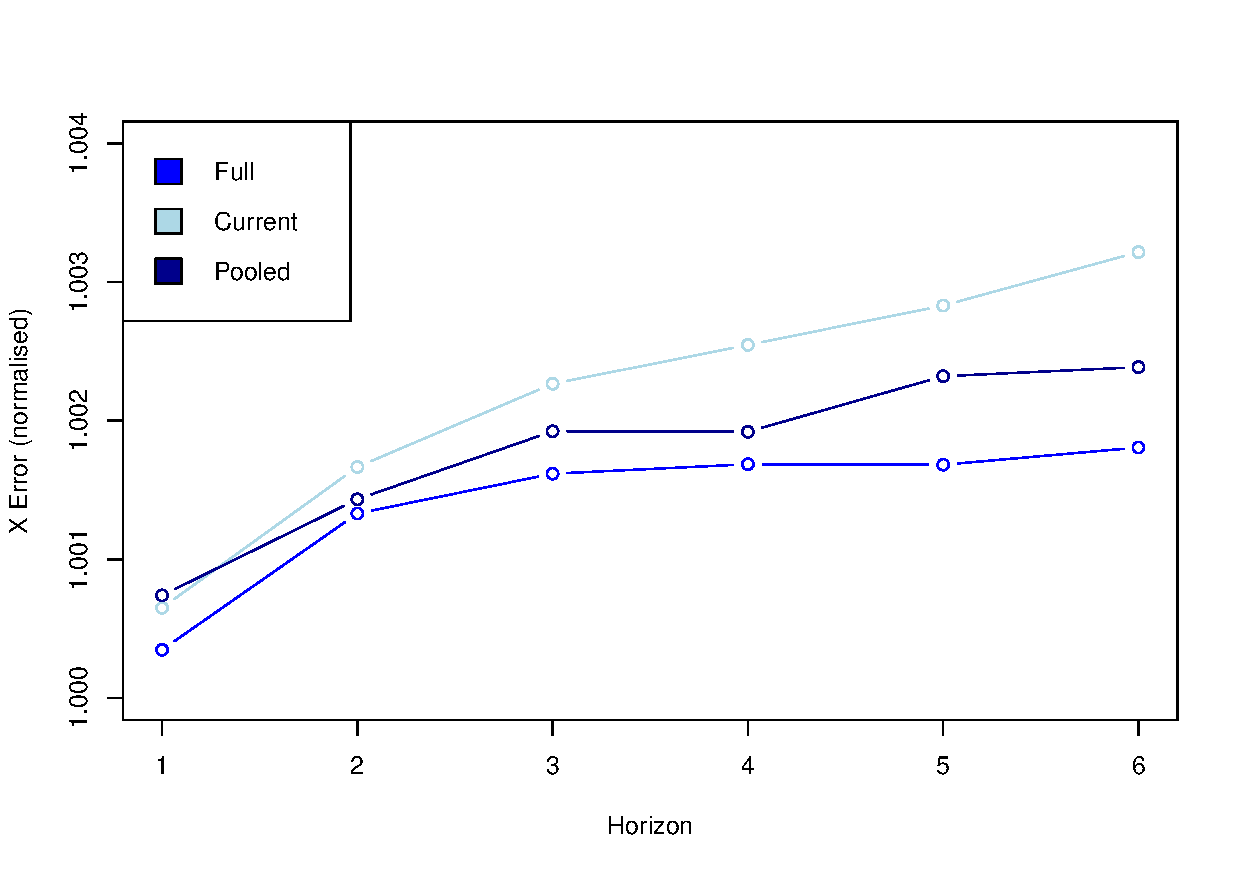
\includegraphics[scale=0.25]{app/appXforecast2.pdf}
	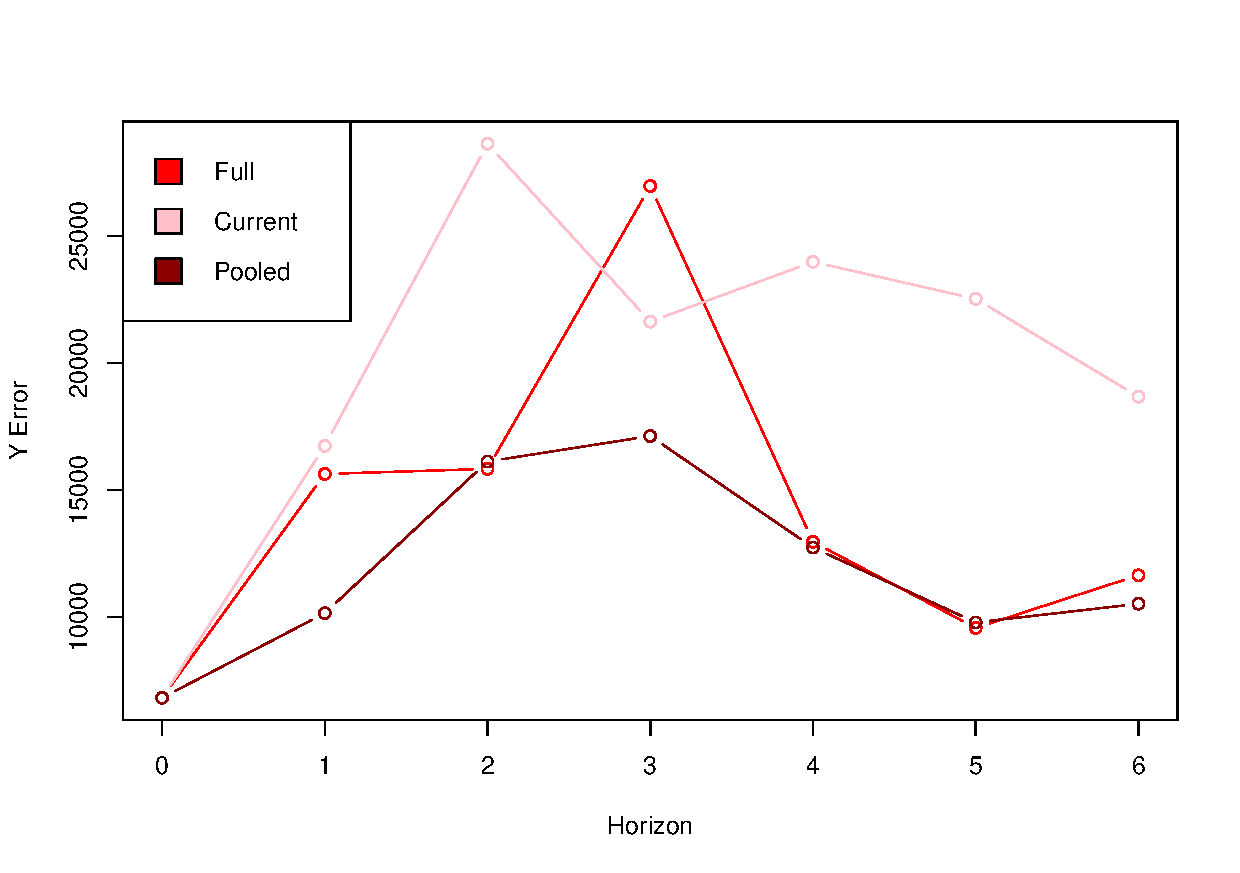
\includegraphics[scale=0.25]{app/appYforecast2.pdf}
	\caption{Forecasts for the panel (left) and GDP (right) up to a 6-step horizon, using different estimation methods}
	\label{fig:appforecasts}
\end{figure}
 \end{frame}
 
 
\begin{frame}{Application: Classifying Recessions}
Classification: $-sign(y_t)$

 Want to control false positives, i.e flagging a recession when there is none, so use $F_{0.5} = \frac{1.25 \cdot precision \cdot recall}{0.25 \cdot precision + recall}$ measure.
 
Paucity of data (lack of positive examples, so \# TP is low or zero) makes comparison/assessment difficult,  still working on this
\end{frame}


\begin{frame}{To Do}

\begin{itemize}
	\item Mathematical proofs (good start, less urgent)
	\item Simulations: compare to existing methods, challenging change types
	\item Online change point detection (trivial in practice, needs mathematical justification)
	\item Classification
	\item \dots
\end{itemize}

\end{frame}


\end{document}